\chapter{Axelrod model for dissemination of culture}

\resp{Miguel Avilés Moreno}


\section{Introduction}

Why don’t all differences in beliefs, attitudes, and behaviors disappear as people interact and become more alike? The Axelrod model, an agent-based model, simulates convergent social influence, where individuals are more likely to adopt traits from similar neighbors. Despite local convergence, global polarization can emerge, influenced by factors like trait count, interaction range, and territory size~\cite{axelrod1997dissemination}. This report simulates the Axelrod model’s key results~\cite{axelrod1997dissemination}, applies it to survey data from the American National Election Studies (ANES)~\cite{anes2025timeseries}, and examines the phase transition from homogeneous to polarized cultural states~\cite{PhysRevLett.85.3536}.

\section{Axelrod Model Description}

The Axelrod model involves $N$ agents as nodes in an interaction network. Each agent $i$ has a state vector of $F$ cultural features: $\sigma_i = (\sigma_{i1}, \sigma_{i2}, \ldots, \sigma_{iF})$, where each $\sigma_{if}$ is one of $q$ integer traits, initially assigned with probability $1/q$. The dynamics proceed as follows:
\begin{enumerate}
    \item Randomly select a connected pair of agents $(i,j)$.
    \item Compute their overlap: $l_{ij} = \sum_{f=1}^{F} \delta_{\sigma_{if}, \sigma_{jf}}$.
    \item If $0 < l_{ij} < F$, agents interact with probability $l_{ij}/F$. During interaction, choose a feature $g$ where $\sigma_{ig} \neq \sigma_{jg}$, and set $\sigma_{ig} = \sigma_{jg}$.
\end{enumerate}
The model has $q^F$ cultural options and reaches consensus if one option dominates the system~\cite{PhysRevLett.85.3536}.

\section{Axelrod Application to ANES Survey}

We apply the Axelrod model to data from the American National Election Studies (ANES) survey, conducted during recent U.S. presidential elections. Four cultural features are selected: gender, party registration, primary election participation, and voting intention, with up to six traits per feature (e.g., voting intention includes six candidate options).

The simulation uses a $19 \times 19$ grid ($N=361$ agents), with $F=4$ features and $q=6$ traits, shown in Figure \ref{ANES_plot}. Initial agent states reflect diverse survey responses. After 2000 iterations, agents form homogeneous groups, reaching a stationary state after 3693 iterations. However, the model’s limitation is evident: simple interactions may not reduce diverse responses to just two dominant cultural states in reality.


\section{Original Axelrod model simulation}

In this section, we evaluate how the number of features ($F$) and the number of traits per feature ($q$) affect the number of cultural regions in the stationary state. Following Axelrod's original approach, we simulated agents on a grid of size $L=10$, assigning initial states uniformly at random. For each combination of $F$ and $q$, the simulation was repeated five times to compute average results. The Table \ref{table:cultural_regions}



The results show that increasing the number of features tends to reduce the number of stable regions and promotes convergence. This occurs because more features increase the probability that neighbors share at least one trait, facilitating interaction. Conversely, increasing the number of traits per feature has the opposite effect, making it more likely that agents will have no shared traits and leading to fragmentation into more distinct cultural regions.

\section{Phase Transition in the Size of the Largest Connected Component}

In this analysis, we explore how the number of traits per feature ($q$) influences the emergence of large homogeneous cultural regions, a phenomenon that can be interpreted as a nonequilibrium order--disorder transition. To quantify this behavior, we define an order parameter as the mean relative size of the largest uniform cultural domain, $\langle S_{\max}\rangle/N$. When $q$ is smaller than a critical threshold value $q_c$, the system tends to reach consensus, resulting in a monocultural state where almost all agents share the same cultural configuration ($\langle S_{\max}\rangle/N \approx 1$). Conversely, for $q > q_c$, the dynamics freeze into a polarized or multicultural state with fragmented domains ($\langle S_{\max}\rangle/N \ll 1$). This transition becomes sharper as the system size increases. In two-dimensional lattices, such as the one used here, the transition is of first order, while in one dimension it becomes continuous. These results are obtained by initializing the system in random, uncorrelated configurations.

The Figure \ref{Phase_Transition} shows the evolution of the order parameter as a function of $q$, illustrating the transition.


For this simulation, we used the following parameters: grid size $L=20$, number of features $F=10$, a maximum of 50,000 sweeps to ensure convergence, and 10 independent runs to average the results. The values of $q$ were varied from 1 to 120 in increments of 5 to cover the region around the critical threshold $q_c$.


\newpage
\section*{Supplementary Materials}

\begin{figure}[htbp]
    \centering
    \begin{minipage}[b]{0.3\textwidth}
        \centering
        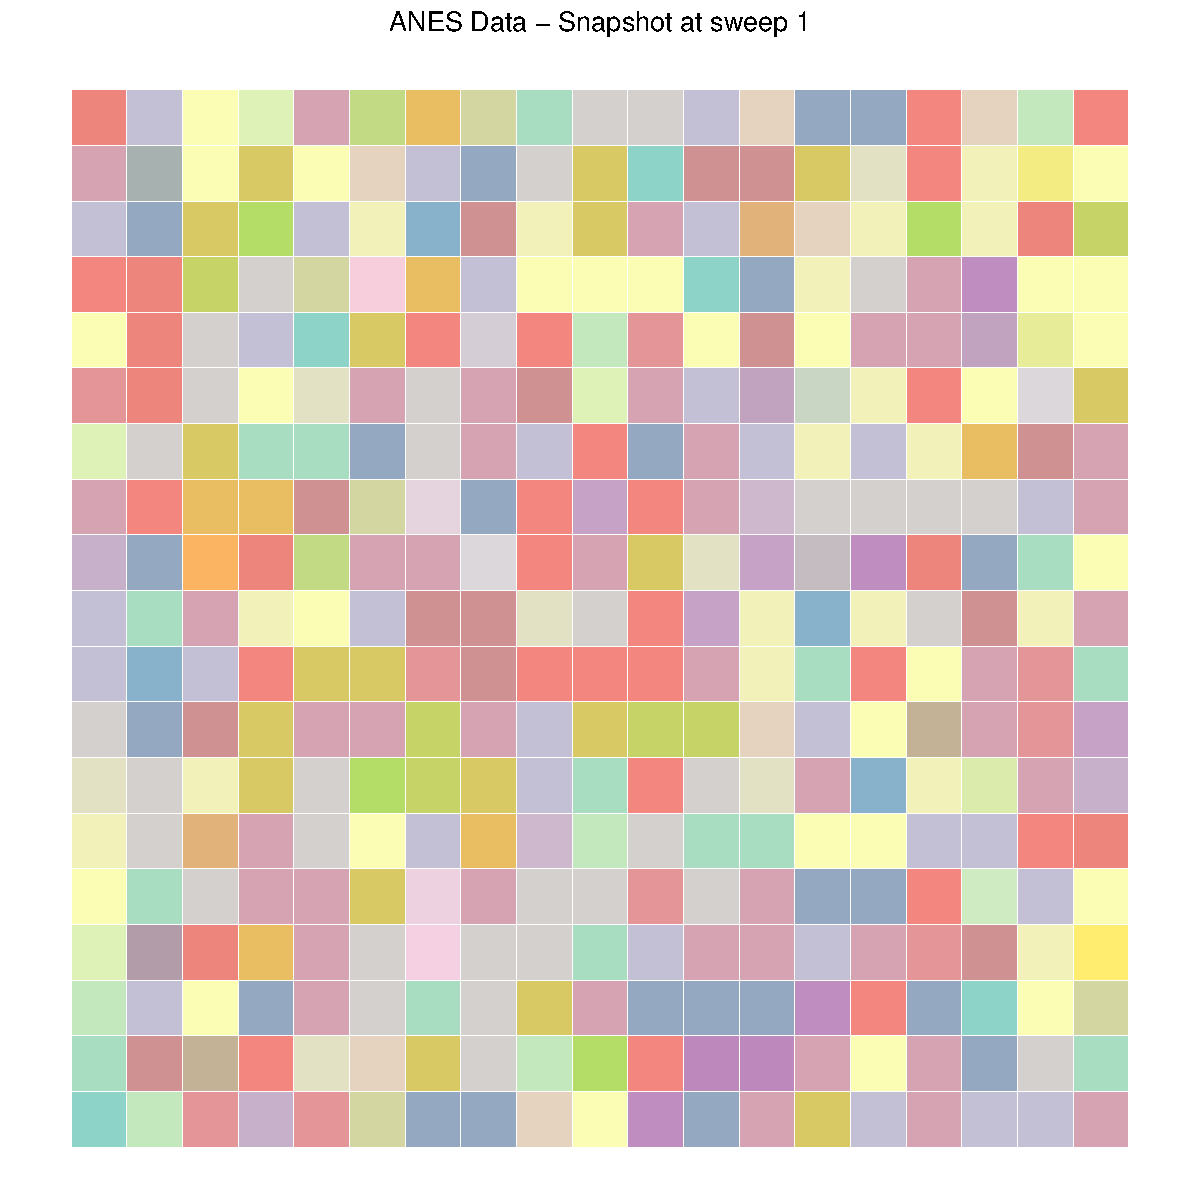
\includegraphics[width=\textwidth]{images/Axelrod_ANES_All_Snapshots-1.pdf}
        \caption*{Iteration 1}
    \end{minipage}
    \hfill
    \begin{minipage}[b]{0.3\textwidth}
        \centering
        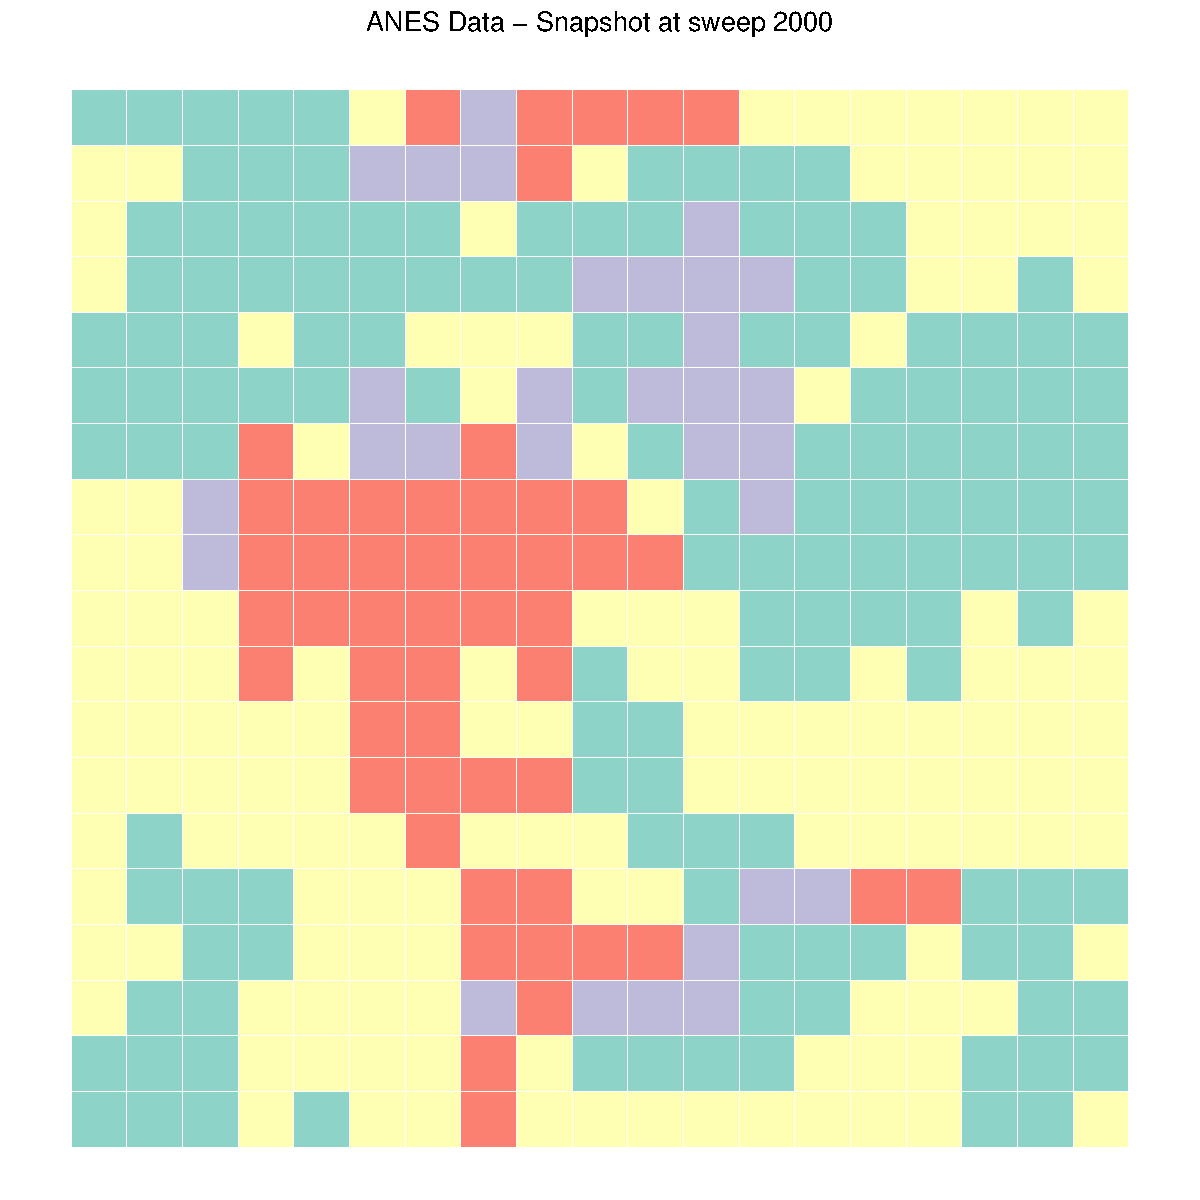
\includegraphics[width=\textwidth]{images/Axelrod_ANES_All_Snapshots-2.pdf}
        \caption*{Iteration 2000}
    \end{minipage}
    \hfill
    \begin{minipage}[b]{0.3\textwidth}
        \centering
        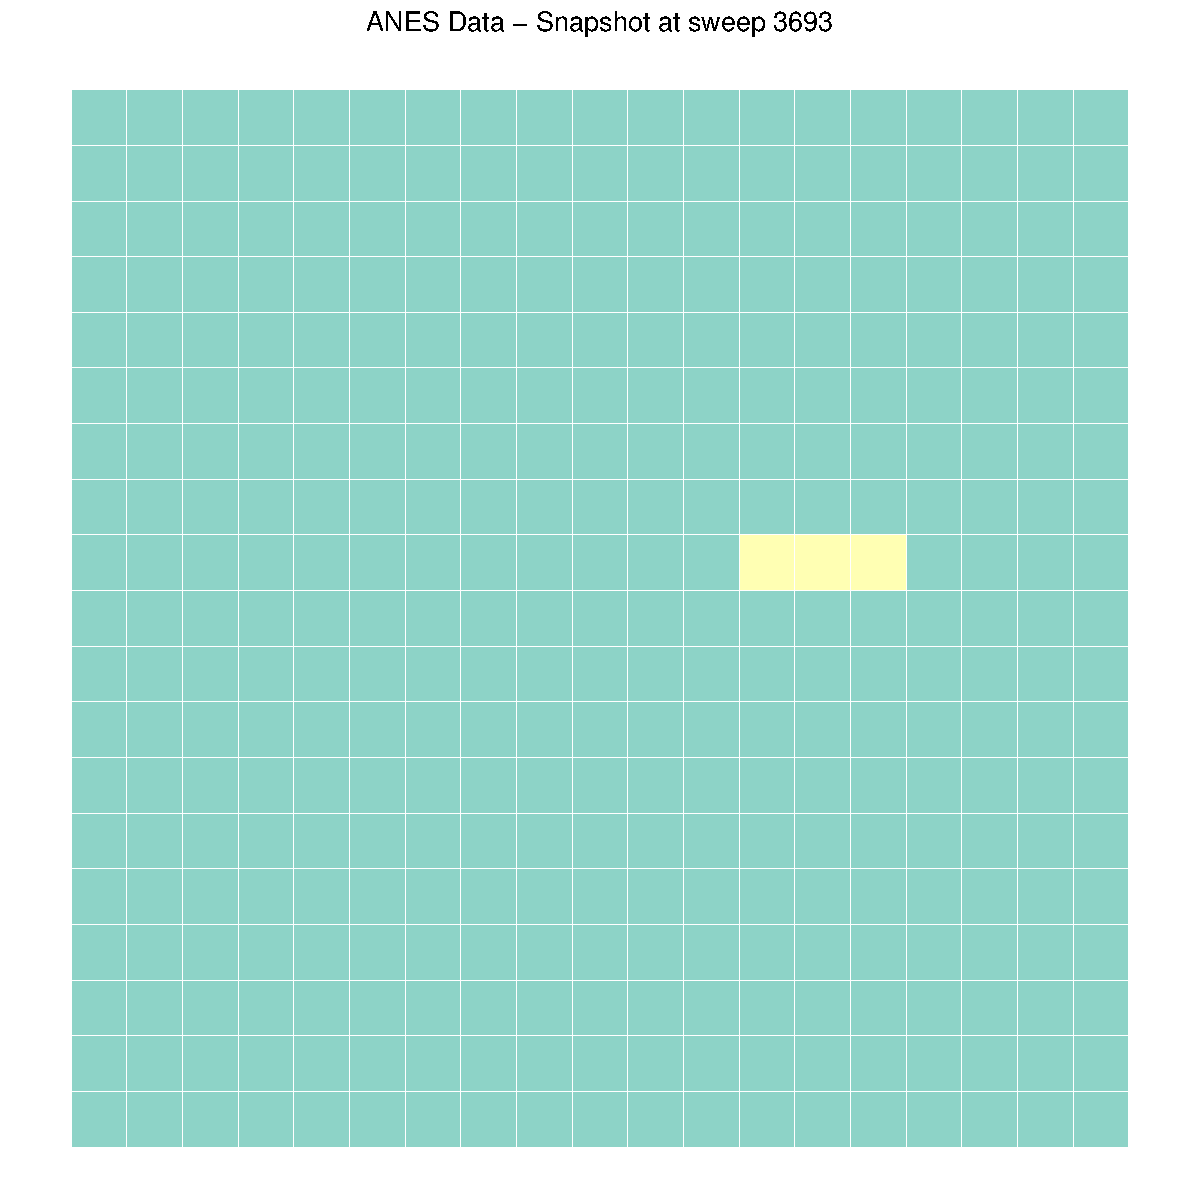
\includegraphics[width=\textwidth]{images/Axelrod_ANES_All_Snapshots-3.pdf}
        \caption*{Iteration 3693}
    \end{minipage}
    \caption{Snapshots of Axelrod model at different iterations (ANES survey).}
    \label{ANES_plot}
\end{figure}

\begin{figure}[h!] 
    \centering
    \begin{minipage}[c]{0.45\textwidth}
        \centering
        \begin{tabular}{c|ccc}
            \toprule
            & $q=5$ & $q=10$ & $q=15$ \\
            \midrule
            $F=5$ & 1.2 & 2.4 & 5.0 \\
            $F=10$ & 1.2 & 1.4 & 1.6 \\
            $F=15$ & 1.2 & 1.6 & 1.8 \\
            \bottomrule
        \end{tabular}
        \captionof{table}{Average number of cultural regions.}
        \label{table:cultural_regions}
    \end{minipage}%
    \hfill%
    \begin{minipage}[c]{0.7\textwidth}
        \centering
        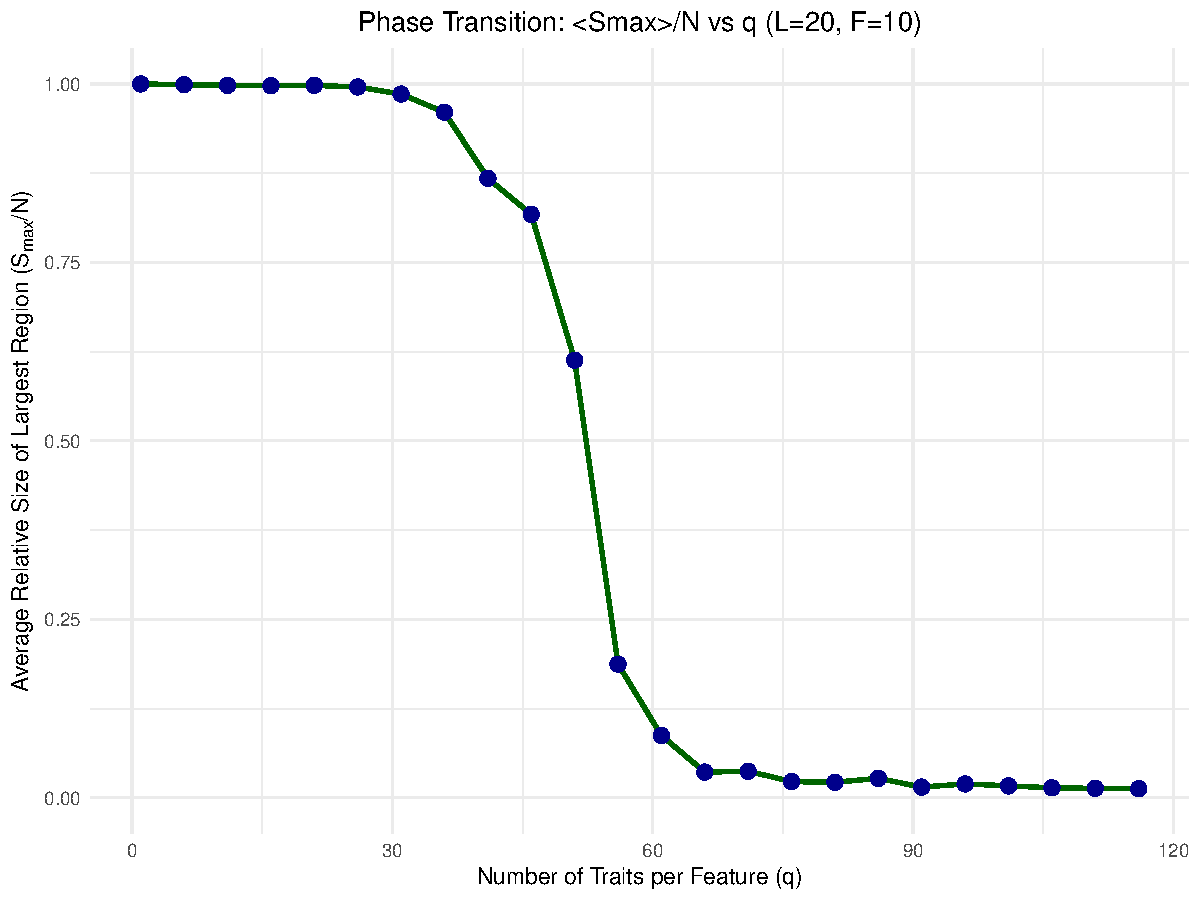
\includegraphics[width=\linewidth]{images/plot_phase_transition.pdf}
        \caption{Relative size of the largest homogeneous region vs. $q$.}
        \label{Phase_Transition}
    \end{minipage}
\end{figure}

\newpage